% !TEX root = main.tex

\chapter{Existing experimental system}
The work developed in this thesis lies on top of an existing experiment. In this chapter we are going to describe the essential parts of the already existing setup on top of which the addressing system has been build. Calcium-40 ions are used in the experiment, the implementation of several techniques for
trapping and manipulating these ions are discussed. Furthermore, the addressing setup utilizes 393 nm light, the laser emitting this light was already installed and used, thus that setup is presented. The experiment can be controlled remotely via computers, an overview of how it is implemented and how it works is also given.

\section{Ion trap and key techniques}
\subsection{Calcium Ions}
\begin{figure}
\centering
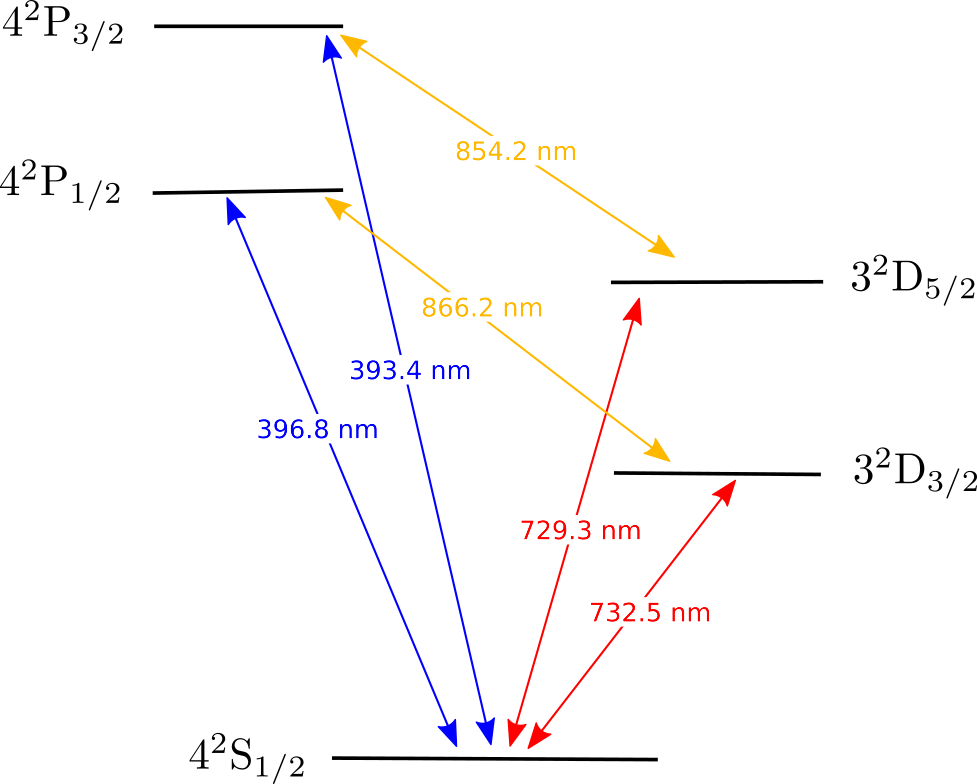
\includegraphics[width = .6 \textwidth]{calciumscheme}
\caption{Level scheme of $^{40}\text{Ca}^+$ with main transitions highlighted. Blue transitions are dipole transitions suitable for cooling, imaging and photon detection. Red transitions are dipole forbidden, but accessible with electric quadrupole, they are used to encode qubits. Orange transition are usually repumped. In addition, the 854 nm transition is tuned in resonance with the cavity for photon generation purposes. From more and precise value see table \ref{transitiontable}}
\label{calciumscheme}
\end{figure}
In choosing the appropriate ion to trap, one looks first of all for simplicity, which means choosing an element with one single electron in the most outer orbital.
This fact limits the choice to the second group of the periodic table, many of these elements has been successfully trapped: beryllium \cite{beryllium}, barium \cite{barium}, strontium \cite{strontium}, and calcium \cite{calcium}.
The latter has been chosen for this experiment, as calcium has transitions easily accessible with commercial diode and titanium-sapphire lasers. The most abundand isotope of calcium is calcium-40, which is a common choice, but not the only one \cite{Tanaka2007}. Nevertheless, $^{40}\text{Ca}^+$ ions were our choice. In figure \ref{calciumscheme} the level scheme of the only electron in the outer shell is presented. A single ground state is present $\text{S}_{1/2}$ with no hyperfine structure as $^{40}\text{Ca}^+$ does not posses a nuclear spin. There are two short lived excited states ($\sim 7$ ns): $\text{P}_{1/2}$, and $\text{P}_{3/2}$ which are accessible with dipole transitions. These states have different decay channel, for $\text{P}_{1/2}$
the branching ratios are $6\%$ to $\text{D}_{3/2}$, and $94\%$ back to the ground state. For  $\text{P}_{3/2}$ there is a probability of $5.3\%$ to decay to   $\text{D}_{5/2}$, $0.6\%$ to go to  $\text{D}_{3/2}$ and $94\%$ to return to  $\text{S}_{1/2}$. Due to the short lifetimes of these two states, they are suitable for laser cooling and state detection, while the states $\text{D}_{3/2}$ and $\text{D}_{5/2}$
are metastable ($\sim 1$ s) since accessible with electric quadrupole transition. Since the lifetime of the D states are much greater than typical coherence time, they can encode a stable qubit and manipulated without worrying about dissipative process. Table \ref{transitiontable} summarizes details about the different transitions, and what they are used for. A more detailed description and implementation is discussed in the next section.

\begin{table}[H]
\centering
\begin{tabular}{c c c c c}
 \toprule
    {Transition} & {wavelength (nm)} & {Decay rate $\Gamma$} & Lifetime $\tau$ & {Main use} \\ \midrule
   $\text{S}_{1/2} \to \text{P}_{1/2}$ & 396.847 & $2\pi \times 20.8$ MHz & 7.7 ns &  Cooling and imaging \\
    $\text{S}_{1/2} \to \text{P}_{3/2}$  & 393.366 & $2\pi \times 21.4$ MHz & 7.4 ns & Photon generation\\ \midrule
   $\text{S}_{1/2} \to \text{D}_{3/2}$ & 732.389 & $2\pi \times 0.132$ Hz & 1.080 s & - \\
    $\text{S}_{1/2} \to \text{D}_{5/2}$  & 729.147 & $2\pi \times 0.136$ Hz & 1.045 s   & Qubit  \\\midrule
    $\text{P}_{1/2} \to \text{D}_{3/2}$  & 866.214 &  $2\pi \times 1.70$ MHz  &  94.3 ns  & Repumping \\
    $\text{P}_{3/2} \to \text{D}_{5/2}$  & 854.209 & $2\pi \times 1.34$ MHz & 101 ns  & Cavity photon  \\
    $\text{P}_{3/2} \to \text{D}_{3/2}$  & 849.802 & $2\pi \times 1.52$ MHz  & 902 ns   & Repumping \\ \bottomrule
\end{tabular}
\caption{Transitions in $^{40}\text{Ca}^+$ and current use in the experiment. Values are taken from \cite{ion_spacing,stute}}
\label{transitiontable}
\end{table}



\subsection{Trapping, cooling, and state readout}
\begin{figure}
\centering
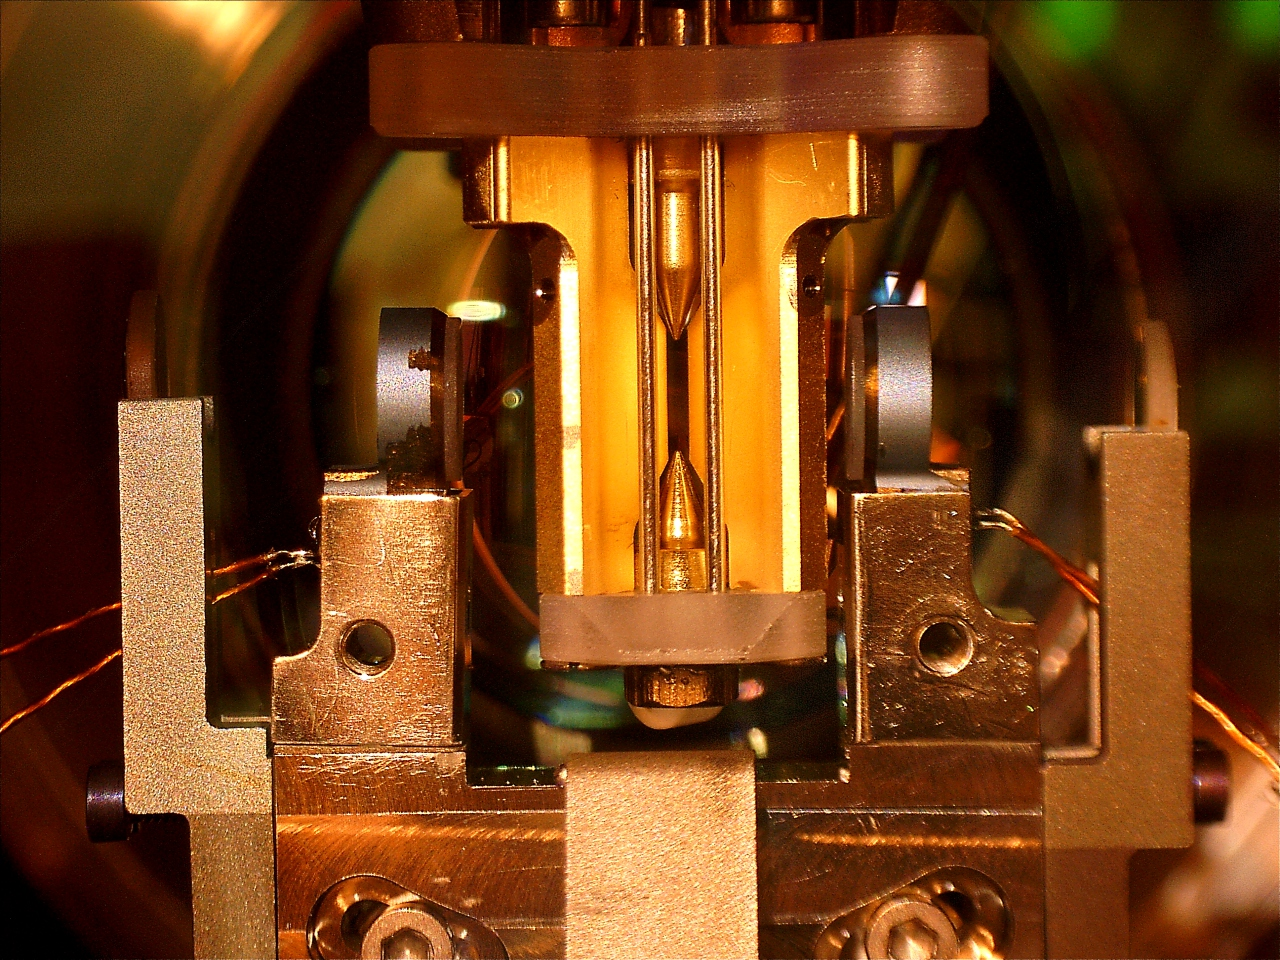
\includegraphics[width = .7\textwidth]{phototrap}
\caption{Photo of the mounted trap, a pair of compensation electrodes and the mirrors of the cavity are also visible.}
\label{trapphoto}
\end{figure}
Our trap is a linear 3D RF Paul trap as depicted in figure (), the picture of the real trap is displayed in figure \ref{trapphoto}. The trap consists of 4 ortoghonal electrodes with blade shape for RF confinement in the radial direction. In the axial direction confinement is achieved with two tip electrodes that forms the endcaps. Everything is made in titanium, it is covered in gold and the trap itself is mounted vertically on a Shappire holder. The endcaps are 5 mm apart, and they are usually kept at a voltage in the order of 500-1000V, which means an axial frequency of $\omega_z \sim 2\pi \times 0.7-1$ MHz. The four blades are 0.8 mm from the center of the trap and driven with an RF of $\sim 24$ MHz. Due to the high power delivered to this blades ($\sim-4$ dBm), the RF signal has to be impedance matched with the trap, this is done with an helical resonator.
The trap also includes three pairs of compensations electrodes that can be used to compensate micromotion.
Loading of ions is done with an atomic oven, calcium is heated a directed towards the trap, in the trap the atoms undergo 2-stage photon ionization. The first laser 375 nm, excite one electron to a very high excited state, the second laser 422 nm, brings the electron to free space ionizing the atom. Such two stage process allows to filter for isotopes and ionize only $^{40}\text{Ca}$. Loading usually takes minutes or tens of minutes depending on the number of ions one wants to load. Storing time can be in the order of days, especially when a single ion is loaded.\\
Once loaded, ions are laser cooled with 397 nm light on the transition $\text{S}_{1/2} \to \text{P}_{1/2}$ detuned at $-\Gamma/2$. An additional repumper on the transition $\text{P}_{3/2} \to \text{D}_{5/2}$ is also used to avoid for the electron being stuck in the $\text{D}_{5/2}$ state. For typical experiment a stage of doppler cooling is always included, this lasts from 1 millisecond up to tens of milliseconds.\\
With the same Doppler cooling light, imaging can also be done. The light shines on the ions exciting the transition $\text{S}_{1/2} \to \text{P}_{1/2}$ driving the electron to the excited states which then decay spontaneously emitting a photons. Photon are collected with a custom objective with NA of $\sim 0.3$, which means an efficiency of 2.5 \% over the solid angle $4\pi$. The objective focuses the collected photons 1.5 meters away where a CCD camera (Andor iXon Ultra 897) is placed. The geometrical path of the imaging is displayed in figure (), the same objective is also used for the addressing setup built within this thesis. Therefore, the imaging optical path must be partially shared with the newly built addressing. In depth overview of objective is therefore given in section ().\\
State read out is possible with this kind of imaging. Consider a qubit encoded in the states
$\text{S}_{1/2} \to \text{D}_{5/2}$, if the imaging laser is switched on, the electron will be projected either to the $\text{S}_{1/2}$ level or in the $\text{D}_{5/2} $. In the first case, photons are scattered from the ion and collected on the camera, in the second case the electron is shelved and will not scatter any photon. Hence, the two cases are distinguishable by counting statistics. An histogram can be constructed  with the number of photon measured, and a properly set threshold differentiates between bright and dark states. Typical detection times are in the order of milliseconds.



\subsection{Photon generations}
- Cavity enhanced Raman transition
\section{393nm laser}
\section{Experiment control}
